% \glsresetall
\chapter{Development of the prototypes} % Main chapter title
\label{Chapter6}

\lhead{Chapter 6. \emph{Development of the prototypes}}

This chapter will provide an overview of the prototype landscapes and explain how the previously introduced technologies were used in them.

\section{Definition of representation}

Before the implementation is showcased, it is explained why and how representation is defined for the context of the thesis.
Since not every micro frontend landscape is the same, a general definition was required before developing the prototypes.
For clarification, the term prototype is a synonym for landscape and vise versa, in the following context.
Those prototypes had to fulfill most of the following requirements, to be considered representative:

\begin{enumerate}
	\item The landscape has to contain at least 6 or more micro frontends
	\item The different micro frontends in the landscape, have to load the same libraries/dependencies to cause redundancies
	\item The tech stack of the landscape has to be heterogenic (not only one UI framework is used).
	\item The embedded micro frontends have to be isolated projects
	\item The landscape contains different versions of a dependency
\end{enumerate}

In specific cases, not all requirements could be met, it is explained why though.

\section{Prototype overviews}

This section will describe the developed prototypes and their respective designs. The whole environment is split over two prototypes, the first of which is the CDN/NPM prototype.
The second prototype, contains the Web Components/WMF landscapes.

\subsection{Prototype 1 - CDN/NPM}

The first prototype developed was the CDN/NPM landscape, totaling 8 micro frontends embedded as iFrames into a Luigi-Core-React application.
Figure \ref{fig:unpkg_prototype_architecture} visualizes this environment.
 
\begin{figure}[!h]
	\centering
	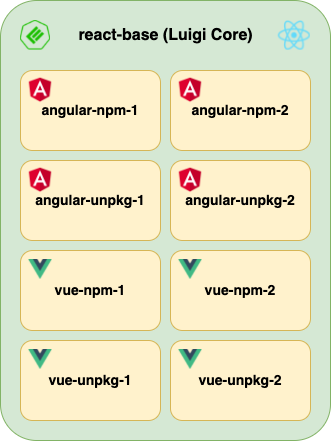
\includegraphics[width=0.7\textwidth]{Figures/unpkg.architecture.drawio.png}
	\caption{Overview of the Luigi prototype using Unpkg.com}
	\label{fig:unpkg_prototype_architecture}
\end{figure}

This prototype represents a Luigi micro frontend landscape, where each Luigi node is a single-page application (SPA). 
The 4 NPM apps, embedded in the landscape, were implemented for comparison. They are meant to show, how the the CDN technology performs, in direct comparison to a bundled application.
In their core, each application contains the same UI-elements. Thus, it is made possible to compare them, in terms of loading times and bytes loaded.
The goals to show with this environment were:

\begin{itemize}
	\item How redundancies occur in a micro frontend landscape
	\item That the browser can´t distinguish between bundled resources, contrary to resources loaded from the CDN
	\item If and what effect the UI framework has on the performance of the site
\end{itemize}

This landscape, fulfills 4 out of the 5 requirements, missing the aspect of different versions. The reason behind this is that, even though it is possible to request different versions of a resource from the CDN, the CDN itself does not offer any means to resolve multiple versions inside the landscape. That means that the library is imported 2 times in different versions. That just increases the redundancies inside the landscape. Due to this predictability, this aspect was not considered for that landscape.

\subsection{Prototype 2 - WMF/Web Components}

The second prototype developed was the WMF and Web Components landscape. It contains 36 micro frontends in total, which are split over 6 Luigi Nodes.
Each Luigi Node, is therefore a compound of micro frontends.
Figure \ref{fig:compound_prototype_architecture} provides an overview of the Node landscape.

\begin{figure}[!h]
	\centering
	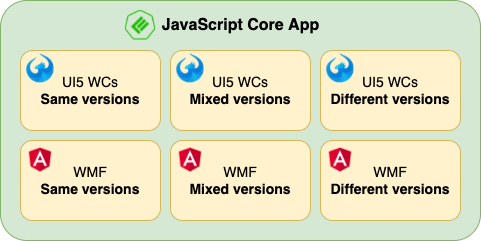
\includegraphics[width=0.7\textwidth]{Figures/compound_views_overview.drawio.png}
	\caption{Overview of the Luigi Nodes in the WMF/Web Components environment}
	\label{fig:compound_prototype_architecture}
\end{figure}

The 6 Nodes displayed in figure \ref{fig:compound_prototype_architecture} contain 6 micro frontends each. 
Figure \ref{fig:compound_wmf_single_node} provides an overview on how the micro frontends are arranged inside a Node into a compound. 

\begin{figure}[!h]
	\centering
	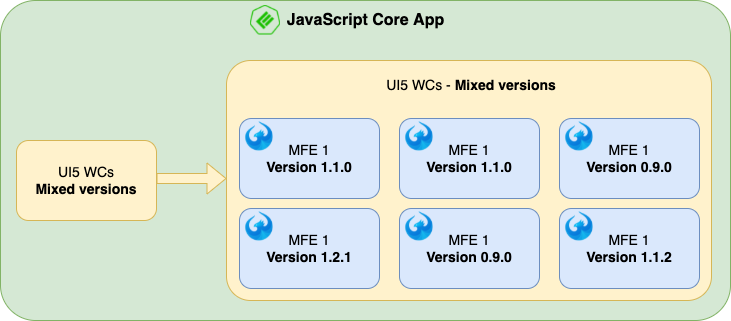
\includegraphics[width=0.7\textwidth]{Figures/compound_wmf_single_node.drawio.png}
	\caption{Example overview of a single Node inside the WMF/Web Components environment}
	\label{fig:compound_wmf_single_node}
\end{figure}

Even though these two technologies are embedded in the same Luigi dashboard, they are referred to as separate landscapes, due to the technological differences.
This prototype fulfills all 5 defined requirements for representation.

The following sections will shortly explain, how the micro frontends are embedded in the Luigi Nodes and showcase the mentioned technological differences.

\subsubsection{Embedding a micro frontend into a compound in Luigi}

The micro frontend compounds for the 3 Web Component Nodes, are created through configurations made in the \texttt{luigi.config.js}.\cite{luigi_wc} \cite{luigi_compound}
Contrary to WMF, these configurations allow to embed the referred compound components in so called \texttt{compoundItemContainer}. The arrangement and number of columns, for the components, inside the Node are defined in the \texttt{luigi.config.js}, too.
Listing \ref{list:compound_luigi_config} shows the exact configuration for that.

\begin{lstlisting}[caption=Configuration of Web Components Node for a compound view, label=list:compound_luigi_config,  xleftmargin=.0\textwidth, xrightmargin=.0\textwidth]
Luigi.setConfig({
	navigation: {
		nodes: [{
			label: 'Home',
			pathSegment: 'home',
			icon: 'home',
			hideFromNav: true,
			globalNav: true,
			hideSideNav: true,
			defaultChildNode: 'mixedVersions',
			children: [
				// Mixed Versions
				{
					label: 'Luigi Compound mixed versions',
					pathSegment: 'mixedVersions',
					icon: 'activate',
					compound: {
						renderer: {
							use: {
								extends: 'grid',
								createCompoundItemContainer: (itemConfig, 
																						containerConfig, 
																						superRenderer) => 
								{
									const itemContainer = superRenderer
									.createCompoundItemContainer(itemConfig);
									if (!itemConfig.noPadding) {
										itemContainer.style = itemContainer
										.getAttribute('style') + 
										' ; padding: 20px ; overflow: hidden';
									}
									return itemContainer;
								}
							},
							config: {
								columns: '1fr 1fr 1fr',
								layouts: [{
									minWidth: 0,
									maxWidth: 1024,
									columns: '3fr',
									gap: 0
								}]
							}
						},
						children: [
						// MFEs for this compound go here
						{
							webcomponent: true,
							viewUrl: 'URL to the view to be embedded',
							label: 'A label for the MFE',
							layoutConfig: {
								column: "auto"
							}
						},
						...
						]
					}
				},
\end{lstlisting}

Line 14 to 16 define the central Node navigation element for the Luigi dashboard. In line 17 it is defined that the content of this Node is a compound. The following line 18 defines the \texttt{renderer} for the content and the tools for it are the properties of the \texttt{use} property in line 19. Line 20 to 34 define the actual CSS attributes of the, to be rendered container for the compound elements. The arrangement of the container , is managed in the \texttt{config} property in line 35. In this scenario, the containers are arranged in 3 columns, each one taking 1 fraction of 1024 pixels.
At line 45 the actual compound elements or micro frontends are defined as an array of JavaScript objects.

\subsubsection{Embedding a micro frontend into a compound in WMF}
\label{embedd_mfe_in_wmf}

Other then the to the Web Component Nodes, the WMF Nodes are actually embedded as iFrames into the Luigi dashboard. Therefore, the Luigi configuration for that landscape, is similar to the CDN/NPM environements. The listing \ref{list:wmf_luigi_config}, shows how it was achieved.

\begin{lstlisting}[caption=Example configuration to embed a WMF micro frontend compound as a Node in Luigi, label=list:wmf_luigi_config,  xleftmargin=.0\textwidth, xrightmargin=.0\textwidth]
	Luigi.setConfig({
		navigation: {
			nodes: [{
				label: 'Home',
				pathSegment: 'home',
				icon: 'home',
				hideFromNav: true,
				globalNav: true,
				hideSideNav: true,
				defaultChildNode: 'sameVersions',
				children: [
                {
					pathSegment: 'wmfHostSame',
					label: 'WMF Compound Same',
					icon: 'technical-object',
					viewUrl: 'https://angular-wmf-same-shell.surge.sh/',
					loadingIndicator: {
						enabled: false
					}
				},
			...
\end{lstlisting}

As it can be seen, the integration is done via an URL. The same view displayed in the dashboard, can be found under the referred URL. This means, to create a compound view in WMF, the creation of the necessary container, the structure and the actual arrangement of the micro frontends, is managed by the host application of the WMF environment and not Luigi.
The code of this development, is shown and explained in section \ref{wmf_implementation_prototype} of this chapter.

\section{CDN - Unpkg.com} 

Chapter \ref{Chapter3}, introduced the concept of the CDN. A remote server is provides the necessary platform resources via an API, thus avoiding the necessity of bundling those resources.
To evaluate the impact of this technology on a micro frontend landscape, the first prototype was developed using the public cloud based CDN Unpkg.com. It is an open-source project, built and maintained by Michael Jackson. It runs on the Cloudflare platform, and auto-scalable servers are provided by Fly.io, which are located in 17 cities around the world.\cite{unpkg_doc}

An open API is available, through which resources can be requested. Via path and query parameters in the URL, necessary information like the dependency version can be provided.

The usage of the Unpkg.com-CDN is embedded in the code. Instead of loading the dependencies via the local \texttt{node\_modules} directory, they are directly loaded using the CDNs API, the usage of which is displayed in the listing \ref{list:unpkg_import}.

\begin{lstlisting}[caption=Import of a dependecy using the unpkg API, label=list:unpkg_import]
	<script src="https://unpkg.com/@ui5/webcomponents@1.0.0-rc.15/dist/StandardListItem.js?module" type="module"></script>
\end{lstlisting}

This script tag is placed in the central \texttt{index.html}. The loaded resource can be read from the URL. The first part of the URL refers to the protocol and the host. The first path parameter is the NPM dependency name. In the case of \ref{list:unpkg_import} it is \texttt{@ui5}, followed by a subdirectory with its respective version annotated with an @.
As it is described in the documentation, the Unpkg.com supports two query parameters \cite{unpkg_doc}.

\begin{itemize}[noitemsep]
	\item \texttt{?meta} - to request meta data about the loaded package, in a JSON format
	\item \texttt{?module} - to expand all import specifiers in JavaScript modules to unpkg URLs
\end{itemize}

If the import is handled via a script tag, as it is done in \ref{list:unpkg_import}, the \texttt{type="module"} attribute has to be added, depending on the resource loaded.
In the case of the given example, the resource is a JavaScript module type. To ensure it is parsed by the runtime as such, this attribute has to be added.\cite{js_module_type}

\section{Web Components - UI5 Web Components} 

The Web Components standard was partially used in the development of the second prototype. For development itself no UI application framework was used, which means all three compounds were developed using plain JavaScript. The actual components used in the micro frontends of the compounds, were taken from a component library called UI5 Web Components. Each element in that library is in fact a Web Component \cite{ui5_wc_github}.
Consisting of the picked elements, and under the usage of the scoping feature of the component library, the 3 compounds where created. The scoping feature in particular, made it possible to scope the tags of the UI5 Web Components, this way a multi-version landscape was simulated.\cite{ui5_webcomponents_scoping}

\begin{lstlisting}[language=JavaScript,caption=Scoping feature used in the prototype, label=list:scoping_wc_prototype,  xleftmargin=.0\textwidth, xrightmargin=.0\textwidth]
import { LuigiElement, html } 
from "@luigi-project/client/luigi-element.js";
import { setCustomElementsScopingSuffix } 
from "@ui5/webcomponents-base/dist/CustomElementsScope.js";
setCustomElementsScopingSuffix("placeholder");
import "@ui5/webcomponents/dist/Dialog.js";
import "@ui5/webcomponents/dist/Button.js";
[...]

export default class extends LuigiElement {
	constructor() {
		super();
		[...]
		render() {
			return html`
			<div>
				<div class="header">
				<h2>Products table - Version: placeholder</h2>
			</div>
			
			<ui5-table-placeholder id="ui5-table" 
			ui5-table sticky-column-header>
			<!-- Columns -->
				<ui5-table-column-placeholder 
				slot="columns" 
				style="width: 4rem">
					<span 
					style="line-height: 1.4rem">
					Product
					</span>
				</ui5-table-column-placeholder>
			
			[...]
			
			</ui5-table-placeholder>
			</div>`;
		}
	}
\end{lstlisting}
	
Listing \ref{list:scoping_wc_prototype} shows the exact usage of the scoping feature. 
The imported \textit{setCustomElementsScopingSuffix} function is used to define a custom suffix, which is applied to all UI5 Web Component elements. Also, as it can be seen in the same listing, the suffix is set to \textit{placeholder} using the imported method \textit{setCustomElementsScopingSuffix("placeholder")}.
This is done for the sake of the experiment itself. It was intended to deploy six similar looking micro frontends, using Web Components, into the Luigi landscape, to test how many redundancies occur. In addition it was meant to be tested how different versions of the same elements could be registered. 
For example, without the scoping feature, a Web Component e.g. the \textit{Bar} element in version \textit{1.0.1} and \textit{1.1.0}, is registered under the same tag name. This causes a conflict, since the registered element might be required in the specific version by a micro frontend. By using the scoping feature, this conflict can be resolved.
Through defining a general version suffix for the elements, they are registered under distinguishable tags in the browser.
In case of the prototype to create this exact scenario, one global tag suffix \textit{placeholder} was picked and later replaced. The replacement itself happened during the bundling of the project. The RollUp bundler provided the necessary functionality for that.
Inside the \texttt{rollup.config.js} several configurations were defined, which are shown in listing \ref{list:rollupconfigjs}.
	
\begin{lstlisting}[language=JavaScript, caption=Content of the \texttt{rollup.config.js}, label=list:rollupconfigjs,  xleftmargin=.0\textwidth, xrightmargin=.0\textwidth]
import resolve from '@rollup/plugin-node-resolve';
import json from '@rollup/plugin-json';
import url from "@rollup/plugin-url";
import { terser } from "rollup-plugin-terser";
import replace from '@rollup/plugin-replace';
import { SameVersions } from './rollup_files/same_version';
import { DiffVersions } from './rollup_files/different_version';
import { MixedVersions } from './rollup_files/mixed_version';

let buildArray = [];

function aggregateConfigs() {
	for(let buildConfig of SameVersions) {
		buildArray.push(buildConfig);
	}
	
	for(let buildConfig of DiffVersions) {
		buildArray.push(buildConfig);
	}
	
	for(let buildConfig of MixedVersions) {
		buildArray.push(buildConfig);
	}
}
	
aggregateConfigs();

export default buildArray;
\end{lstlisting}
	
The configuration of the bundler was split into several JavaScript files, to improve the readability of the file itself. The content of such a file can be seen in listing \ref{list:rollupconfigfile}.
	
\begin{lstlisting}[language=JavaScript, caption=Configuration content for the \texttt{rollup.config.js}, label=list:rollupconfigfile, xleftmargin=.0\textwidth, xrightmargin=.0\textwidth]
import resolve from '@rollup/plugin-node-resolve';
import json from '@rollup/plugin-json';
import url from "@rollup/plugin-url";
import { terser } from "rollup-plugin-terser";
import replace from '@rollup/plugin-replace';

export const MixedVersions = [
// 1
{
	input: 'src/tableView.js',
	output: {
		file: 'dist/tableViewMixedVersions1.js',
		format: 'es',
		compact: true
	},
	plugins: [
	replace({
		'placeholder': '0-9-0',
	}),
	terser(),
	resolve(),
	json(),
	url({
		limit: 0,
		include: [
		/.*assets\/.*\.json/,
		],
		emitFiles: true,
		fileName: "[name].[hash][extname]",
		publicPath: "\" + new URL(\".\", import.meta.url) + \"", // relative configuration for assets (TBD with UI5 Web Components team)
	})
	]
},
// 2
{
	input: 'src/tableView.js',
	output: {
		file: 'dist/tableViewMixedVersions2.js',
		format: 'es',
		compact: true
	},
	plugins: [
	replace({
		'placeholder': '1-1-0',
	}),
	terser(),
	resolve(),
	json(),
	url({
		limit: 0,
		include: [
		/.*assets\/.*\.json/,
		],
		emitFiles: true,
		fileName: "[name].[hash][extname]",
		publicPath: "\" + new URL(\".\", import.meta.url) + \"", // relative configuration for assets (TBD with UI5 Web Components team)
	})
	]
},
[...]
]
\end{lstlisting}
	
The file, which is bundled for each configuration, in the shown listing \ref{list:rollupconfigfile}, is always the same. This can be taken from the \texttt{input} property. The bundling result though, is named differently, which can be read from the \texttt{output} property. The first bundle result is called \texttt{tableViewMixedVersions1.js}, the second \texttt{tableViewMixedVersions2.js} etc.
The \texttt{replace} method, in e.g. line 17, of the first configuration object, replaces a string inside the input file. In the shown case, the string \textit{placeholder} is first replaced with \textit{0-9-0} and in line 43 with \textit{1-1-0}. 
This results in, the elements to be named differently, inside those files. Thus, they are later registered under different tags in the browser. In this case, elements registered by the first bundled micro frontend, are called for example \texttt{<ui5-bar-0-9-0>} and for the second then \texttt{<ui5-bar-1-1-0>}.

One file is bundled several time. Each bundle result, has a different name and replaces the placeholder string with a different string. This way, multiple micro frontends can be generated, which then again register the same elements under differently named tags. Therefore, those elements are treated as new elements.

\section{Webpack Module Federation with Angular} 
\label{wmf_implementation_prototype}

The three implemented versions for the the WMF landscape are similar to one another, the only difference can be found are the dependencies and their configured sharing. Listing \ref{list:wmf_sameversions_shell} shows the configuration for the \textit{sameVersions} Node.

\begin{lstlisting}[language=JavaScript, caption=Content of \texttt{webpack.config.js} of the shell of the sameVersions WMF project, label=list:wmf_sameversions_shell, xleftmargin=.0\textwidth, xrightmargin=.0\textwidth]
[...]
module.exports = {
	[...]
	plugins: [
	new ModuleFederationPlugin({
		name: "shell",
		filename: "remoteEntry.js",
		shared: share({
			"@angular/core": { 
				singleton: true, 
				strictVersion: false, 
				requiredVersion: '= 12.2.0'
			},
			"@angular/common": { 
				singleton: true, 
				strictVersion: false, 
				requiredVersion: '= 12.2.0' 
			},
			...sharedMappings.getDescriptors()
		})
		
	}),
	sharedMappings.getPlugin()
	]};
\end{lstlisting}

As it is shown, the shared dependencies are defined in between lines 22 and 24. Line 18 and 19 define the name of the application in the landscape and the name of the file after bundling. For the above case, it has to be mentioned that the remotes are separate applications in their own runtime. Therefore, they have to be imported via the network, thus no \texttt{remote} property is configured in this file. To add the dynamically loaded remotes, a service had to be developed which imports the remotes at runtime \cite{wmf_angular_dynamicfederation}. This service is shown in listing \ref{list:wmf_lookup_service}.

\begin{lstlisting}[language=JavaScript, caption=Content of \texttt{lookup.service.ts} for remote module loading in shell applications, label=list:wmf_lookup_service,  xleftmargin=.0\textwidth, xrightmargin=.0\textwidth]
[...]
@Injectable({ providedIn: 'root' })
export class LookupService {
	lookup(): Promise<PluginOptions[]> {
		return Promise.resolve([
		{
			remoteEntry: 'https://angular-wmf-same-mfe1.surge.sh/remoteEntry.js',
			remoteName: 'mfe1',
			exposedModule: './Mfe1',
			
			displayName: 'Mfe1',
			componentName: 'Mfe1Component'
		},
		[...]	
		] as PluginOptions[]);
	}
}
\end{lstlisting}

This service serves the information of the remotely loaded modules to a proxy plugin, which is responsible for the actual rendering of the components. This proxy plugin creates the container, as some sort of placeholder for the remotes. \cite{wmf_angular_dynamicfederation}
\newpage
\begin{lstlisting}[language=JavaScript, caption=Content of \texttt{plugin-proxy.component.ts} for remote module loading in shell applications, label=list:wmf_pluginproxy,  xleftmargin=.0\textwidth, xrightmargin=.0\textwidth]
	[...]	
	@Component({
		selector: 'plugin-proxy',
		template: `
		<ng-container #placeHolder></ng-container>
		`
	})
	export class PluginProxyComponent implements OnChanges {
		@ViewChild('placeHolder', { read: ViewContainerRef, static: true })
		viewContainer: ViewContainerRef;
		
		constructor(
		private injector: Injector,
		private cfr: ComponentFactoryResolver) { }
		
		@Input() options: PluginOptions;
		
		async ngOnChanges() {
			this.viewContainer.clear();
			
			const Component = await loadRemoteModule(this.options)
			.then(m => m[this.options.componentName]);
			
			const factory = this.cfr.resolveComponentFactory(Component);
			const compRef = this.viewContainer.createComponent(factory, null, this.injector);		
		}
	}
\end{lstlisting}

Line 8 of listing \ref{list:wmf_pluginproxy} defines the \texttt{ng-container} with the identifier called \texttt{placeholder}. This identifier is used in the code below to select and actually fill the container with a remote module. The functionality is placed in one of Angulars Lifecycle hook methods \texttt{ngOnChanges}, which is triggered when changes to input properties occur \cite{wmf_angular_lifecyclehooks}.
In there, the container is first cleared, then a remote loading option is selected from the array of the \texttt{lookup.service.ts}. The following line, creates an Angular component out of the loaded remote and inserts it into the placeholder container, using the imported dependencies.
The type \texttt{PluginOptions}, was defined in an interface, exporting a type definition. The code for it, is displayed in listing \ref{list:wmf_plugintype}.
\newpage
\begin{lstlisting}[language=JavaScript, caption=Content of \texttt{plugin.ts} for remote module loading in shell applications, label=list:wmf_plugintype,  xleftmargin=.0\textwidth, xrightmargin=.0\textwidth]
import { LoadRemoteModuleOptions } from '@angular-architects/module-federation';
export type PluginOptions = LoadRemoteModuleOptions & {
	displayName: string;
	componentName: string;
};
\end{lstlisting}

The previously imported \texttt{@angular-architects/module-federation} dependency offers an existing type interface for that use case. This type, is extended by two more properties in line 4 and 5 of listing \ref{list:wmf_plugintype}.

By configuring the above service and component, it is made possible to load federated modules via the network into the host application.
The configuration for a federated module (aka remote) can be seen in listing \ref{list:wmf_sameversions_mfe1}.

\begin{lstlisting}[language=JavaScript, caption=Content of \texttt{webpack.config.js} of the mfe1 remote app of the same versions WMF project, label=list:wmf_sameversions_mfe1,  xleftmargin=.0\textwidth, xrightmargin=.0\textwidth]
[...]
module.exports = {
	[...]
	plugins: [
	new ModuleFederationPlugin({
		name: "mfe1",
		filename: "remoteEntry.js",
		exposes: {
			'./Mfe1': './src/app/mfe1.component.ts'
		},
		shared: share({
			"@angular/core": { 
				singleton: true, 
				strictVersion: false, 
				requiredVersion: '<= 12.2.0' 
			},
			"@angular/common": { 
				singleton: true, 
				strictVersion: false, 
				requiredVersion: '<= 12.2.0' 
			},
			"@fundamental-ngx/core": { 
				singleton: true, 
				strictVersion: false,
				requiredVersion: '0.33.0-rc.214' 
			},
			...sharedMappings.getDescriptors()
		})
	}),
	sharedMappings.getPlugin()
	]};
\end{lstlisting}

As mentioned in chapter \ref{Chapter5}, to share dependencies every remote has to participate. Therefore, similarities can be found in the sharing configurations of the remotes and hosts. 
Between line 7 and 11, the actual federation of the module is configured. The reference to the module is later bundled in a file with the name, defined in the \texttt{filename} property, in this case it is \texttt{remoteEntry.js}.
This is the file, which is automatically generated when the remote is compiled and serves as the entry point for the application when it is loaded into the host. Therefore, this is the file accessed via the server URL in the \texttt{lookup.service.ts} \ref{list:wmf_lookup_service}.
As soon as the script is loaded via the service, the exposed module paths and names become known to the host and can be used to load the module \cite{wmf_concepts}. Thus the \texttt{expose} property contains a JavaScript object, which maps the path to the actual component. In the shown case, it is mapped to \texttt{./Mfe1}.

In section \ref{embedd_mfe_in_wmf}, it was shown how the developed WMF Nodes are embedded in the Luigi dashboard. The shown snippets in this section have shown how a compound of micro frontends is created using WMF. In direct comparison with the Luigi compounds, it becomes obvious, that WMF does not really offer support for heterogenic landscapes. This is shown indirectly in the implemented prototype, but can be applied to any WMF landscape, too. 
The first indicator is, the necessity of a separate service and plugin, for the dynamic loading and rendering of the remotes.

Additionally, the only reason this prototype was implemented without conflicts is, because each remote is actually an Angular project/component. If for instance, one project would be a VueJS based remote, the integration of it would be connected to more obstacles. This can be showcased, in lines 21 and 24 of the plugin proxy from listing \ref{list:wmf_pluginproxy}, which responsible to load a remote component into the created container. The methods used in those lines, expect an Angular component. If now a VueJS remote would be loaded into, a conflict occurs.

Furthermore, routing inside a compound view of WMF, requires further workarounds, even in a homogenic landscape. In the case of the implemented prototype, the routers of the Angular micro frontends are not shared with the other members of the compound. Therefore, a router would have to be either loaded via an API or a dynamic import by the other participants or else routing between the micro frontends is impossible.
Additionally, enabling the \texttt{webpack.config.js} and with it the Module Federation, is different for every framework. In case of Angular, it was achieved via the installation of the mentioned dependencies.
